% This LaTex file's purpose is to draw a flow chart representing PyVVO's 
% main loop, which can be found in app.py.

\documentclass[tikz]{standalone}
\usetikzlibrary{shapes.geometric, arrows.meta, fit, calc, positioning, automata, decorations.pathreplacing}

% Declare the layers
% https://tex.stackexchange.com/a/75498/208656
\pgfdeclarelayer{background}
\pgfsetlayers{background,main}

% tikzset for flowcharts.
% https://tex.stackexchange.com/a/342227/208656
% Reference for label shifting in style:
% https://tex.stackexchange.com/a/78690/208656
\tikzset{flowchart/.style = {
	base/.style = {
		draw=black,
		very thick,
		inner sep=10pt,
		outer sep=0pt,
		text width=10.0cm,
		minimum height=0.8cm,
		align=flush center,
	},
	labelshift/.style = {
		prefix after command= {\pgfextra{\tikzset{every label/.style={xshift=0.42cm}}}}
	},
	startstop/.style = {
		base,
		labelshift,
		rectangle,
		rounded corners,
		fill=red!30
	},
	io/.style = {
		base,
		trapezium,
		trapezium left angle=70,
		trapezium right angle=110,
		trapezium stretches=true,
		fill=blue!30,
	},
	process/.style = {
		base,
		labelshift,
		rectangle,
		fill=orange!30
	},
	decision/.style = {
		base,
		diamond,
		aspect=1.2,
		fill=green!30
	},
	arrows.meta/.style = {
		very thick,
	 	-{Stealth[]}
	}
}}

\begin{document}

% Shortcut for inline code:
% https://stackoverflow.com/a/21344989
\newcommand{\code}[1]{\texttt{#1}}

% Label counter for the flow chart.
\newcounter{ac}
\renewcommand{\theac}{\alph{ac}}
\newcommand{\ac}[1]{(\refstepcounter{ac}\alph{ac})\label{#1}}

% To put parentheses around references:
\newcommand{\acref}[1]{(\ref{#1})}

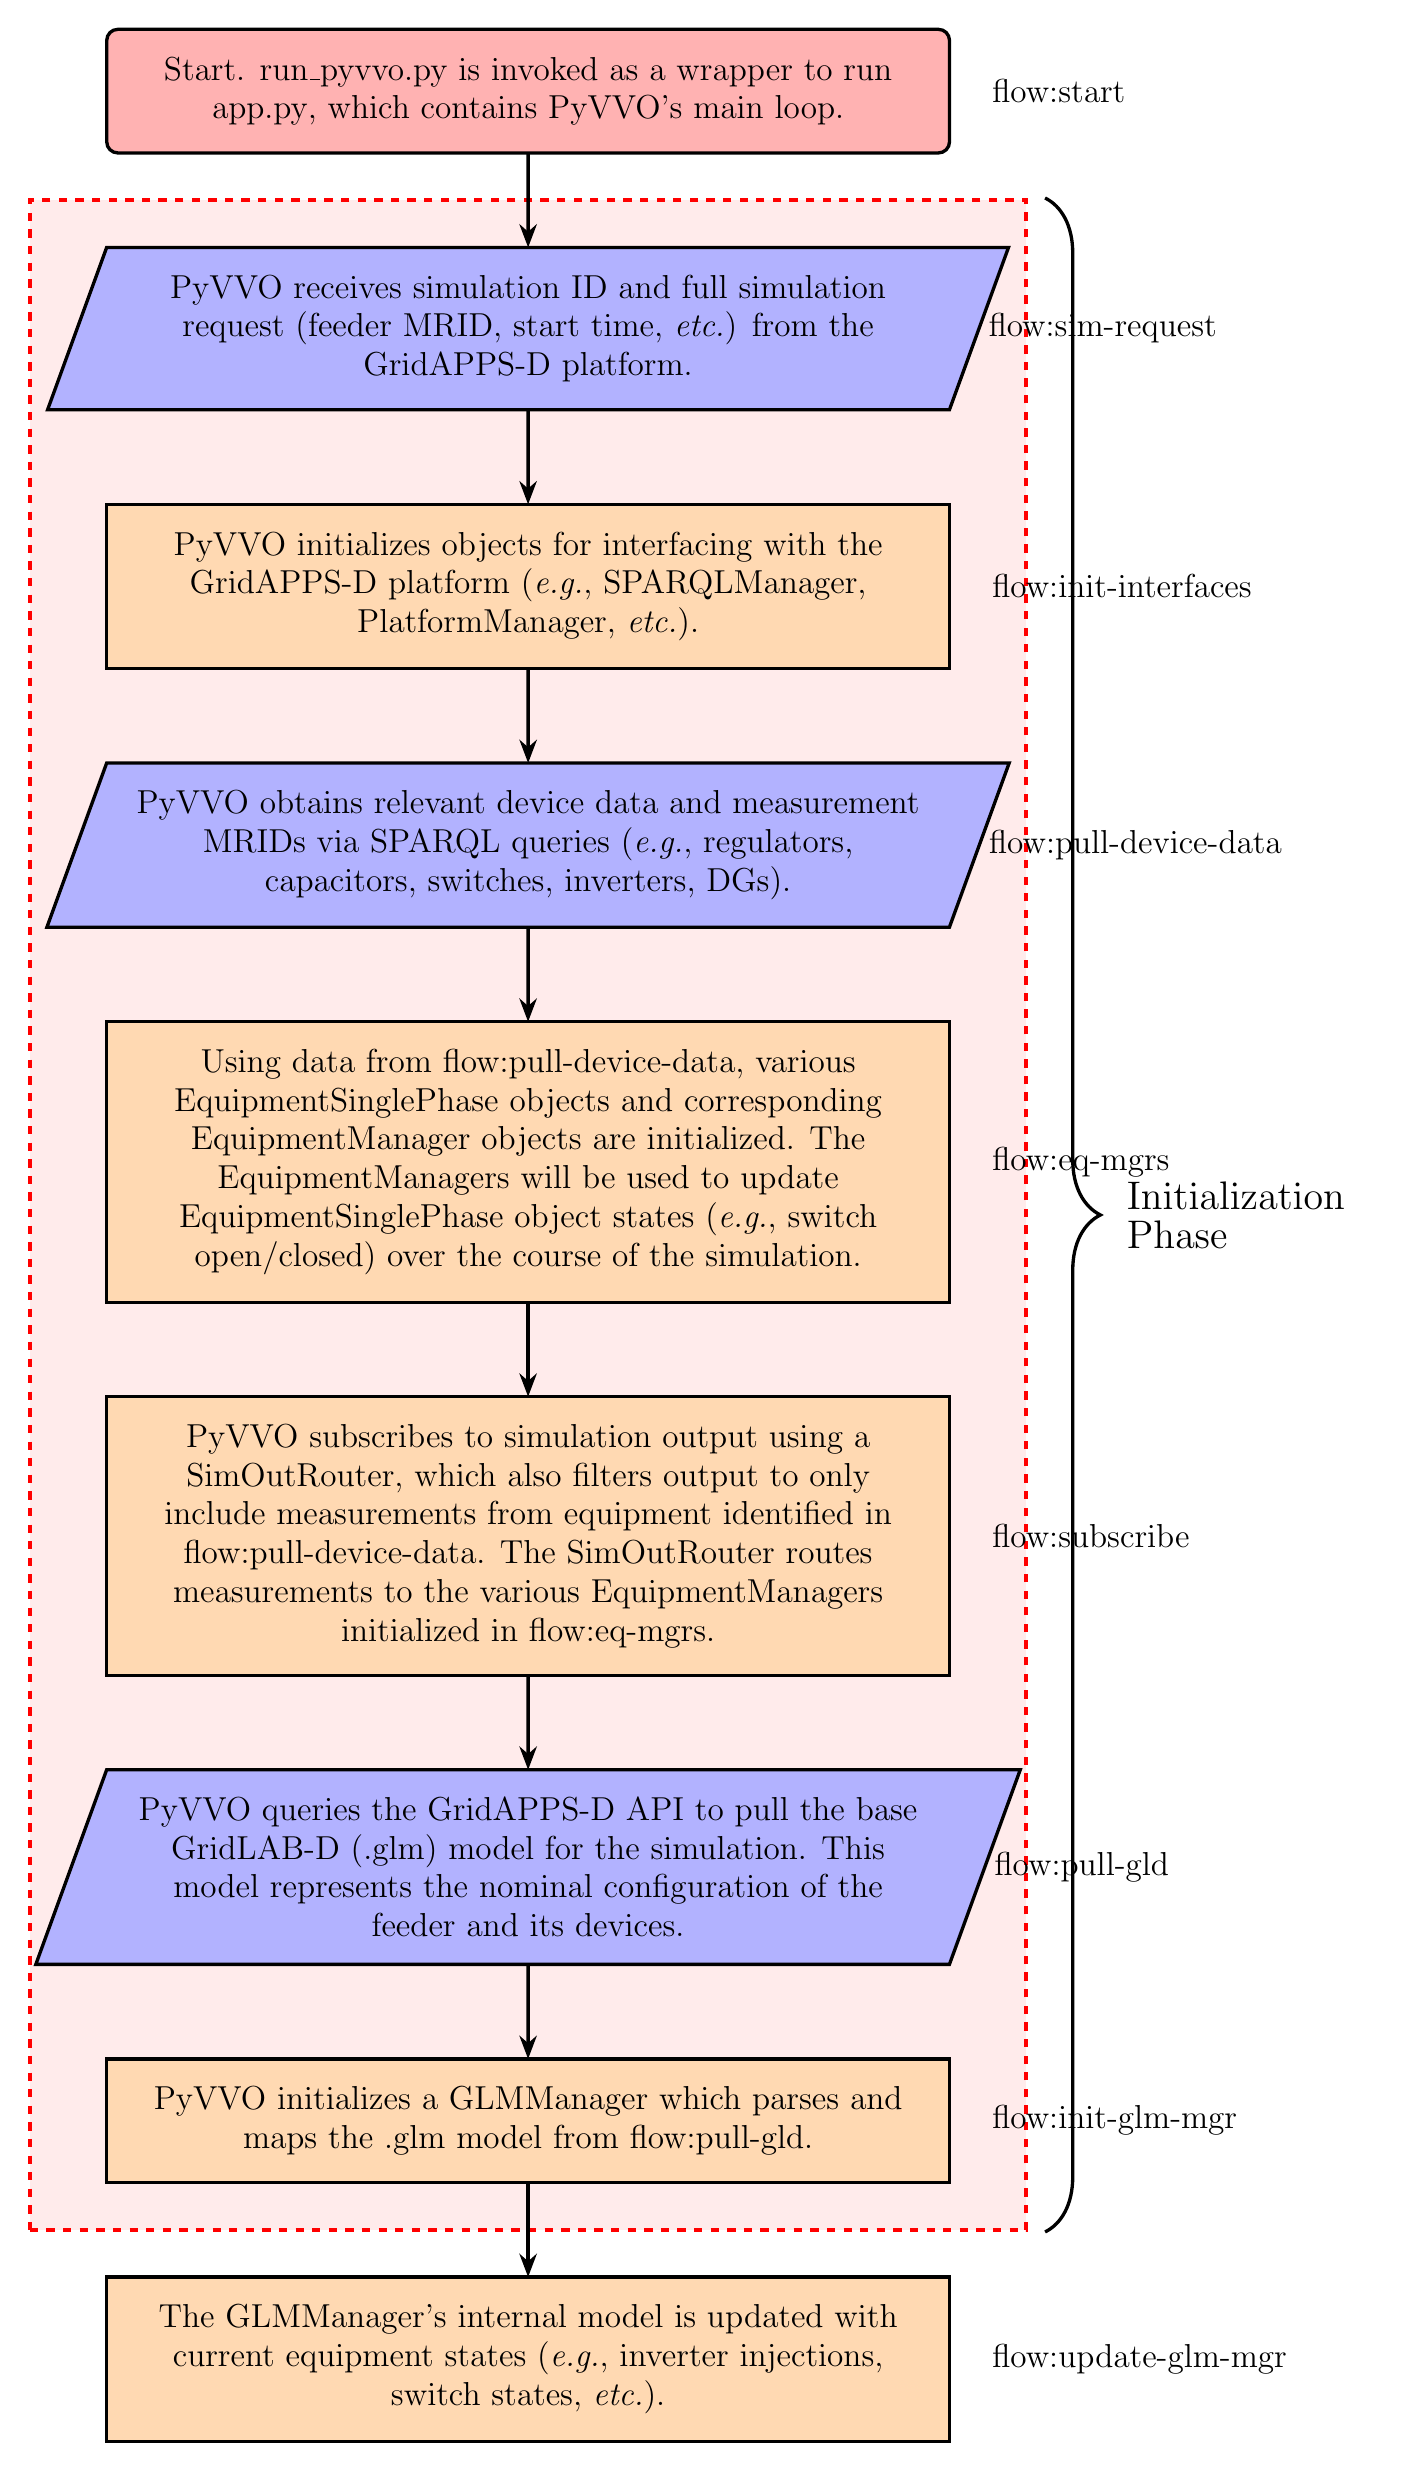
\begin{tikzpicture}[flowchart, node distance=1.2cm] 
% \begin{tikzpicture}
% , outer sep=2cm
\tikzstyle{every node}=[font=\large]
	% note the difference between below of=   and below=of:
	% https://tex.stackexchange.com/q/9386/208656

	%%%%%%%%%%%%%%%%%%%%%%%%%%%%%%%%%%%%%%%%%%%%%%%%%%%%%%%%%%%
	% NODES
	%%%%%%%%%%%%%%%%%%%%%%%%%%%%%%%%%%%%%%%%%%%%%%%%%%%%%%%%%%%
	\node (start)
	[startstop, label={right:\ac{flow:start}}]
	{Start. \code{run\_pyvvo.py} is invoked as a wrapper to run \code{app.py},
	which contains PyVVO's main loop.};
	%
	\node (sim-request)
	[io, below=of start, label={right:\ac{flow:sim-request}}]
	{PyVVO receives simulation ID and full simulation request
	(feeder MRID, start time, \textit{etc.}) from the GridAPPS-D platform.};
	%
	\node (init-interfaces)
	[process, below=of sim-request, label={right:\ac{flow:init-interfaces}}]
	{PyVVO initializes objects for interfacing with the GridAPPS-D platform
	(\textit{e.g.}, \code{SPARQLManager}, \code{PlatformManager}, \textit{etc.}).};
	%
	\node (pull-device-data)
	[io, below=of init-interfaces, label={right:\ac{flow:pull-device-data}}]
	{PyVVO obtains relevant device data and measurement MRIDs via SPARQL queries
	(\textit{e.g.}, regulators, capacitors, switches, inverters, DGs).};
	%
	\node (eq-mgrs)
	[process, below=of pull-device-data, label={right:\ac{flow:eq-mgrs}}]
	{Using data from \acref{flow:pull-device-data}, various
	\code{EquipmentSinglePhase} objects and corresponding
	\code{EquipmentManager} objects are initialized. The 
	\code{EquipmentManager}s will be used to update
	\code{EquipmentSinglePhase} object states (\textit{e.g.},
	switch open/closed) over the course of the simulation.};
	%
	\node (subscribe)
	[process, below=of eq-mgrs, label={right:\ac{flow:subscribe}}]
	{PyVVO subscribes to simulation output using a \code{SimOutRouter},
	which also filters output to only include measurements from equipment
	identified in \acref{flow:pull-device-data}. The \code{SimOutRouter} routes
	measurements to the various \code{EquipmentManager}s initialized in
	\acref{flow:eq-mgrs}.};
	%
	\node (pull-gld)
	[io, below=of subscribe, label={right:\ac{flow:pull-gld}}]
	{PyVVO queries the GridAPPS-D API to pull the base GridLAB-D (\code{.glm}) model for the simulation.
	This model represents the nominal configuration of the feeder and its devices.};
	%
	\node (init-glm-mgr)
	[process, below=of pull-gld, label={right:\ac{flow:init-glm-mgr}}]
	{PyVVO initializes a \code{GLMManager} which parses and maps the \code{.glm} model from
	\acref{flow:pull-gld}.};
	%
	\node (update-glm-mgr)
	[process, below=of init-glm-mgr, label={right:\ac{flow:update-glm-mgr}}]
	{The \code{GLMManager}'s internal model is updated with current equipment states
	(\textit{e.g.}, inverter injections, switch states, \textit{etc.}).};
	%
	%%%%%%%%%%%%%%%%%%%%%%%%%%%%%%%%%%%%%%%%%%%%%%%%%%%%%%%%%%%
	% ARROWS
	%%%%%%%%%%%%%%%%%%%%%%%%%%%%%%%%%%%%%%%%%%%%%%%%%%%%%%%%%%%
	% Add layers as per https://tex.stackexchange.com/a/75498/208656
	\begin{pgfonlayer}{main}
		\draw[arrows.meta] (start) -- (sim-request);
		%
		\draw[arrows.meta] (sim-request) -- (init-interfaces);
		%
		\draw[arrows.meta] (init-interfaces) -- (pull-device-data);
		%
		\draw[arrows.meta] (pull-device-data) -- (eq-mgrs);
		%
		\draw[arrows.meta] (eq-mgrs) -- (subscribe);
		%
		\draw[arrows.meta] (subscribe) -- (pull-gld);
		%
		\draw[arrows.meta] (pull-gld) -- (init-glm-mgr);
		%
		\draw[arrows.meta] (init-glm-mgr) -- (update-glm-mgr);
	\end{pgfonlayer}

	% Background layer.
	\begin{pgfonlayer}{background}
		% Draw a box around all the initialization data.
		% https://tex.stackexchange.com/a/75498/208656
		\node (init-box) [
			draw=red, fit= (sim-request) (init-glm-mgr), inner sep=0.6cm,
			ultra thick, dashed, fill=red!20, fill opacity=0.4
		] {};
		% \coordinate (init-se) at (init-box.south east);

	\end{pgfonlayer}

	% Draw a curly brace.
	\draw [decorate, very thick, decoration={brace, amplitude=20pt, raise=6pt, mirror}]
	(init-box.south east) -- (init-box.north east)
	node [black, midway, xshift=2.75cm, text width=3cm] {\Large Initialization Phase};
	
\end{tikzpicture}
\end{document}